
\documentclass[12pt]{article}
\usepackage{scrextend}
\usepackage[utf8]{inputenc}
\usepackage[polish]{babel}
\usepackage[T1]{fontenc}%polskie znaki
\usepackage[utf8]{inputenc}%polskie znaki
\usepackage{geometry}
\usepackage{float}
\usepackage{enumitem}
\usepackage{hyperref}
\usepackage{graphicx}
\usepackage{tabulary}
\usepackage{etoc}
\usepackage[normalem]{ulem} 
\usepackage{tikz}
\usepackage[bf]{caption}
\usepackage{amsmath}

\renewcommand{\baselinestretch}{1.5}

\usepackage{listings}
\usepackage{xcolor}
\usepackage[
    backend=bibtex,
    style=numeric
  ]{biblatex} 

\definecolor{codegreen}{rgb}{0,0.6,0}
\definecolor{codegray}{rgb}{0.5,0.5,0.5}
\definecolor{codepurple}{rgb}{0.58,0,0.82}
\definecolor{backcolour}{rgb}{0.95,0.95,0.92}
 
\lstdefinestyle{mystyle}{
    backgroundcolor=\color{backcolour},   
    commentstyle=\color{codegreen},
    keywordstyle=\color{magenta},
    numberstyle=\tiny\color{codegray},
    stringstyle=\color{codepurple},
    basicstyle=\ttfamily\footnotesize,
    breakatwhitespace=false,         
    breaklines=true,                 
    captionpos=b,                    
    keepspaces=true,                 
    numbers=left,                    
    numbersep=5pt,                  
    showspaces=false,                
    showstringspaces=false,
    showtabs=false,                  
    tabsize=2
}
\renewcommand{\lstlistlistingname}{Spis listingów}\lstset{style=mystyle}

\graphicspath{ {img/} }
\newgeometry{lmargin=2.0cm, rmargin=2.0cm, tmargin=2.0cm, bmargin=2.0cm}
\clubpenalty=9996
\widowpenalty=9999
\brokenpenalty=4991
\predisplaypenalty=10000
\postdisplaypenalty=1549
\displaywidowpenalty=1602

\title{ 
    \vspace*{50mm}
    \textsc{
        \textbf{Rozpoznawanie i przetwarzanie obrazów}\\
        \large Śledzenie stanu stołu bilardowego 
    }
} 
\author{
Damian Koper,  241292\\
Mateusz Gurski, 242089
}

\date{\today}
\bibliography{literature}
\begin{document}

\maketitle

\newpage
\setcounter{tocdepth}{2}
\localtableofcontents
\listoffigures
\lstlistoflistings
\vfill
Repozytorium projektu: \url{https://github.com/damiankoper/ripo}
\newpage

\section{Cel projektu}
Celem projektu było stworzenie systemu umożliwiającego śledzenie stanu stołu podczas gry w bilard. Stan stołu obejmuje pozycję i numer bil obecnych na stole, jak i tych znajdujących się w łuzach. Obejmuje on również pozycje kija gracza.

\subsection{Cele dodatkowe}
Dodatkowym celem było rozpoznanie gracza aktualnie wykonującego ruch oraz zliczanie punktów i sygnalizowanie błędów i fauli.

\section{Stół bilardowy}

Kluczowym elementem projektu jest stół bilardowy. Na etapie projektowania systemu przyjęto następujące założenia dotyczące kamery i stołu:

\begin{enumerate}[noitemsep]
    \item Kamera jest umieszczona nad stołem, prostopadle do płaszczyzny stołu.
    \item Stół musi w całości zawierać się w kadrze zgodnie z orientacją kadru. Nie ma znaczenia jednak przesunięcie i obrót obrazu ($\pm45^\circ$).
    \item Stół musi być dobrze i jednolicie oświetlony.
    \item Przed rozpoczęciem działania systemu, po zmianie pozycji kamery, system musi wykonać proces inicjalizacji, który wymaga usunięcia wszystkich elementów ruchomych ze stołu.
\end{enumerate}

Ze względu na sytuację epidemiczną na terenie Polski w czasie prowadzenia prac nad projektem, nie było możliwości uzyskania dostępu do żadnego stołu, przeprowadzania i nagrania rozgrywki. Posiłkowano się nagraniami rozgrywek dostępnymi w serwisie YouTube z ustawieniami kamery spełniającymi wymagania\cite{youtube}.

\section{Przepływ danych i architektura}

Stworzony system składa się z dwóch głównych komponentów:
\begin{itemize}[noitemsep]
    \item VideoProcessor
    \item PoolVD
\end{itemize}

Komponent \textit{VideoProcessor} zajmuje się przetwarzaniem wideo i komunikacją z komponentem \textit{PoolVD}. Pozyskuje on obraz dostarczony poprzez strumieniem używającym protokołu UDP. Nie użyto tutaj protokołu TCP, ponieważ analiza stołu powinna odbywać się w czasie rzeczywistym i rozwiązanie to wprowadziłoby dodatkowy element synchronizacji, który mógłby mieć wpływ na dostarczany obraz.

Źródłem obrazu może być klip wideo wysyłany z użyciem narzędzie \textit{ffmpeg}, albo obraz na żywo z kamery RaspberryPI. Oba te rozwiązania zostały przetestowane. Wykorzystanie strumienia sieciowego jako źródła obrazu jest rozwiązaniem uniwersalnym, ponieważ oferuje stabilny interface po stronie komponentu \textit{VideoProcessor}.

Komponent \textit{VideoProcessor} jest równocześnie serwerem obsługującym połączenia zgodne z protokołem WebSocket. Umożliwia to na szybkie dostarczanie danych wyjściowych do dowolnej liczby klientów. Umożliwia to również na opartą na zdarzeniach komunikację pomiędzy klientami wyświetlającymi dane, omówioną w dalszej części sprawozdania. Protokół WebSocket, w przeciwieństwie do HTTP do dwukierunkowej komunikacji wykorzystuje zawsze jeden strumień.

Przepływ danych od materiału wideo do użytkownika zobrazowane zostało na diagramie z rysunku \ref{dataflow}.


\begin{figure}[h]
    \centering
    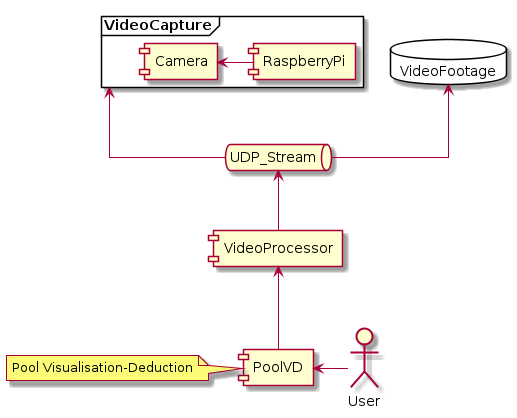
\includegraphics[width=10cm]{./diagrams/out/data_flow.png}
    \caption{Przepływ danych.}
    \label{dataflow}
\end{figure}

\subsection{Architektura}

Detekcja, klasyfikacja, wyświetlania i dedukcja są złożonymi procesami używającymi wiele zasobów sprzętowych. Jednym z filarów sprawnego działania systemu jest sprawny przepływ danych i wielokrotne używanie produktów pośrednich tego przetwarzania. Aby uzyskać płynność przetwarzanego obrazu i optymalne wykorzystanie zasobów wykorzystano podejście wielowątkowe połączone z asynchronicznością.

\subsection{Komponent VideoProcessor}

\begin{figure}[h]
    \centering
    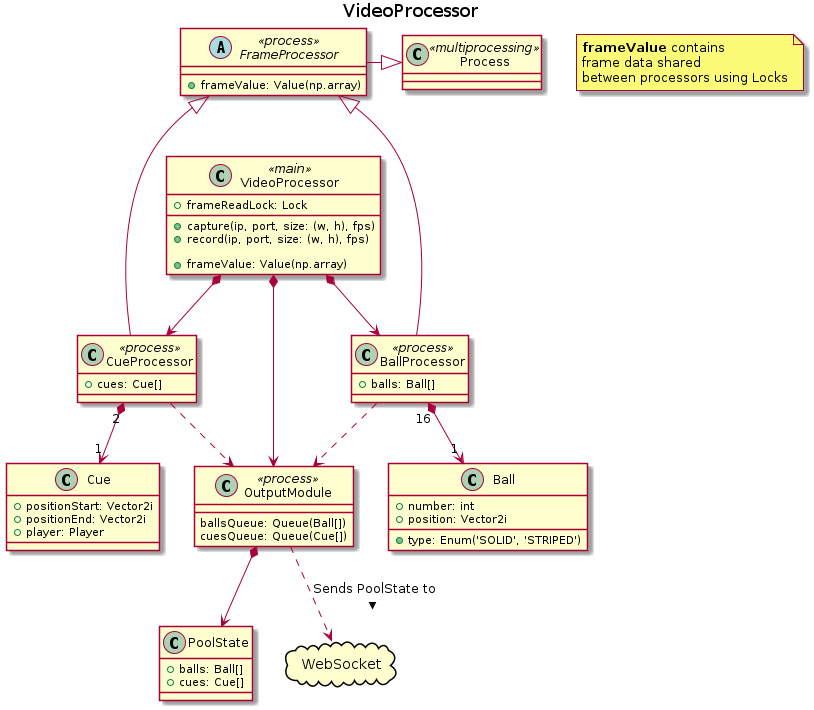
\includegraphics[width=14cm]{./diagrams/out/video_processor_cd.png}
    \caption{Diagram klas komponentu VideoProcessor.}
    \label{vp_cd}
\end{figure}

Punktem wejścia programu jest moduł \lstinline{main}. Przyjmuje on argumenty określające jego działanie - parametry strumienia wejściowego oraz tryb pracy. Może on zostać uruchomiony w trybie domyślnej analizy obrazu lub w celu jego nagrania. Dalszy opis tyczy się trybu analizy obrazu.

Działanie przetwarzania klatki bazuje na działaniu trzech głównych klas - procesów systemowych, nazwanych procesorami. Każdy z nich posiada swój rozbudowany obiekt konfiguracji. Ogólną strukturę klas komponentu przedstawia diagram na rysunku~\ref{vp_cd}.

\begin{enumerate}
    \item \textbf{VideoProcessor}. Nazwa taka sama jak nazwa całego komponentu. Klasa odpowiedzialna za odebranie klatki i oddanie sterowania do klasy \lstinline{InitialFrameProcessing} w celu wykonania procesu inicjalizacji i wstępnego przetworzenia klatki. Po wstępnym przetworzeniu umieszcza ona produkty tego przetwarzania klatki w zmiennych współdzielonych pomiędzy innymi klasami - procesorami.
    \item \textbf{BallProcessor}. Klasa odpowiedzialna za detekcję i klasyfikację bil. W celu klasyfikacji wykrytych bil klasa ta przekazuje sterowanie do klasy \lstinline{Classification}.
    \item \textbf{CueProcessor}. Klasa odpowiedzialna za detekcję kija. %TODO MAti jak się się zmieniło to dopisz tu ogólnie
\end{enumerate}

Procesy \textbf{BallProcessor} i \textbf{CueProcessor} przed rozpoczęciem przetwarzania oczekują na klatkę, jeśli nie jest ona dostępna. Dzięki funkcjonowaniu zmiennych współdzielonych, w których przekazywane są klatki przez \textbf{VideoProcessor}, oba procesory w momencie rozpoczęcia przetwarzania pobierają zawsze aktualne dane. Pozwala to na przetwarzanie niezależnie od wydajności algorytmów w poszczególnych klasach.

Po zakończeniu przetwarzania każdej klatki \textbf{BallProcessor} i \textbf{CueProcessor} wysyłają wynik swoich działań w postaci obiektów \lstinline{Ball} lub \lstinline{Cue} do kolejek modułu OutputModule.



\subsubsection{OutputModule}

OutputModule jest osobnym procesem, który obsługuje trzy procedury:
\begin{enumerate} [noitemsep]
    \item Serwer komunikacji zewnętrznej - \lstinline{WebSocketServer}.
    \item Obserwator kolejki wykrytych bili.
    \item Obserwator kolejki wykrytych kii.
\end{enumerate}

\begin{figure}[h]
    \centering
    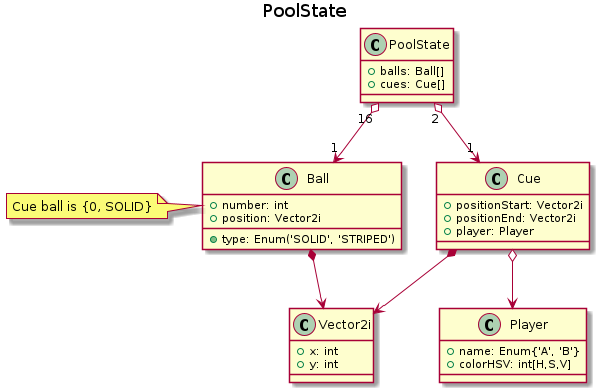
\includegraphics[width=10cm]{./diagrams/out/pull_state_cd.png}
    \caption{Struktura PoolState.}
    \label{poolstate}
\end{figure}

Moduł zawiera również ostatni aktualny wykryty stan stołu. Strukturę te prezentuje diagram na rysunku nr \ref{poolstate}.
Obserwatory obserwujące kolejkę, po umieszczeniu w nich danych przez moduły \textbf{BallProcessor} i \textbf{CueProcessor} aktualizują obiekt \lstinline{PoolState} i wymuszają wysłanie stanu stołu do klientów przez serwer.

Protokół WebSocket umożliwia komunikację full-duplex w dowolny sposób. W celu ustandaryzowania komunikacji pomiędzy klientami, a serwerem zdecydowano się wybrać zorientowaną zdarzeniowo bibliotekę Socket.IO \cite{socket.io}.

% TODO Damian: Opisać Eventy

\section{Detekcja i klasyfikacja}
% TODO Wszystko zaczyna się w Videoprocessor tu się pozyskuje obraz i robi wstępny proces jego przetwarzania - wycinanie itd, to jak wycinać i co wysłać dalej jest ustalane w procesie inicjalizacji
\subsection{Proces inicjalizacji}
% Uśrednianie klatki
% detekcja stoł↓
% Polepszanie macierzy transformacji
% Ważne - zaznaczyć, że inicjalizacja działa nawet po jednej klatce, tylko im więcej tym lepiej
% możę skrinki z zaznaconym wykrytym stołem

\subsection{Produkty przetwarzania wstępnego}
% tutaj skrinki możę ze 2 tej średniej klatki i obecnej wyciętej
% pamiętaj o \ref w tekście i [h] to latex to ładnie ułoży

\subsection{Bile}
%cały proces opisać BP

\subsection{Kij}

%cały proces opisać CP

\section{Wyświetlanie i dedukcja}
% TODO Damian
\section{Uruchomienia systemu}
% TODO Damian
\section{Podsumowanie i wnioski}
% TODO Damian
\newpage

\printbibliography

\end{document}